%%%%%%%%%%%%%%%%%%%%%%%%%%%%%%%%%%%%%%%%%%%%%%%%
%
% Strath PhD Thesis Template
%	by Jethro Browell [jethro.browell@strath.ac.uk]
%
%	Guidelines for thesis format, submission and content are found in
%	General and Course Regulations for Graduate and Postgraduate
%	Awards and Degrees, section 20.6.
%
%	Using .eps or .pdf is recomended to prduce high quality figures etc.
%
%	The Strathclyde logo can be found in other formats at www.strath.ac.uk.
%
%%%%%%%%%%%%%%%%%%%%%%%%%%%%%%%%%%%%%%%%%%%%%%%%

\documentclass[a4paper,oneside,11pt]{book}

% bold symbols
\newcommand{\betabb}{\boldsymbol{\beta}}
\newcommand{\nablabb}{\boldsymbol{\nabla}}
\newcommand{\gammabb}{\boldsymbol{\gamma}}
\newcommand{\sigmabb}{\boldsymbol{\sigma}}

% Pauli matrices
\newcommand{\sx}{\sigma^x}
\newcommand{\sy}{\sigma^y}
\newcommand{\sz}{\sigma^z}

% AGP-related commands
\newcommand{\dlambda}{\partial_{\lambda}}
\newcommand{\AGP}[1]{\mathcal{A}_{#1}}
\newcommand{\adj}[1]{#1^{\dagger}}
\newcommand{\dotlambda}{\dot{\lambda}}
\newcommand{\approxAGP}{\Bar{\AGP{\lambda}}}

% Other mathsy things
\newcommand{\HCD}{H_{\rm CD}}
\newcommand{\R}{\mathbb{R}}
\newcommand{\C}{\mathbb{C}}

% Formatting stuff + comments
\newcommand{\acrref}[1]{\hyperref[acr:#1]{#1}}
\newcommand{\reminder}[1]{\textcolor{blue}{Reminder: #1}}

% Some help with writing pseudocode
\makeatletter
\def\BState{\State\hskip-\ALG@thistlm}
\makeatother

\usepackage{amsbsy}
\usepackage{amsmath}
\usepackage{amsfonts}
\usepackage{graphicx}
\usepackage{multirow}
\usepackage{mathrsfs}
\usepackage{color}
\usepackage[hidelinks]{hyperref}
\usepackage{cite}
\usepackage{enumitem}
\usepackage{epsfig}
\usepackage{caption}
\usepackage{subcaption}
\usepackage{physics}
\usepackage[strict]{changepage}

%own macros

% Page Margins - Strath Requirement
\usepackage[left=4cm,right=2.5cm,top=2cm,bottom=4cm,includehead,includefoot,headheight=15pt]{geometry}

% Page Headers
\usepackage{fancyhdr}
\fancyhf{}
\renewcommand{\headrulewidth}{0pt} % optional
%\fancyhead[L]{\nouppercase{\leftmark} \hfill Section \nouppercase{\rightmark}}
\fancyhead[L]{\nouppercase{\leftmark}}
\cfoot{\thepage}
\pagestyle{fancy}

% Draft Watermark
\usepackage[draft=true,allpages=true,fontfamily=cmr,angle=90,scale=0.1,mark={\fboxsep=35pt\fboxrule=0pt\relax\fbox{-- DRAFT -- \today~--}},xcoord=-80,ycoord=-20]{util/draftmark}


% Line Spacing
%\def\baselinestretch{1.5} 
\usepackage{setspace}
\setstretch{1.5}

% Place UoS Logo on Title Page (this package modifies the "\maketitel" command.)
\usepackage{titling}
\pretitle{%
  \begin{flushright}
  \vspace{-9.5cm}
%  
\includegraphics[width=5cm,natwidth=472,natheight=531]{logo} \\[7cm]
  
\includegraphics[width=5cm]{images/logo} \\[6cm]
  \end{flushright}
  \begin{center}
  \LARGE
  \posttitle{\end{center}}}

\title{Counterdiabatic, Better, Faster, Stronger: \\
\normalsize{Overcoming Losses in Quantum Processes} \\ PhD Thesis}
\author{Ieva \v{C}epait\.{e}
\\ \small Quantum Optics and Quantum Many-Body Physics\\[-0.8ex]
\small Department of Physics\\[-0.8ex]
\small University of Strathclyde, Glasgow\\
}




%%%%%%%%%%%%%%%%%%%%%%%%%%%%%%%%%%%%%%%%%%%%%%%%%%%%%%%%%%%%%%
\begin{document}

\maketitle


%%%%%%%%%%%%%%%%%%%%%%%%%%%%%%%%%%%%%%%%%%%%%%%%%%%%%%%%%%%%%%
\frontmatter
%%%%%%%%%%%%%%%%%%%%%%%%%%%%%%%%%%%%%%%%%%%%%%%%%%%%%%%%%%%%%%

% Declaration
\topskip0pt
\vspace*{\fill}
\noindent
\begin{quote}
	\centering
	This thesis is the result of the author's original research. It has been composed by the author and has not been previously submitted for examination which has led to the award of a degree. \\[5pt]
	%
	The copyright of this thesis belongs to the author under the terms of the United Kingdom Copyright Acts as qualified by University of Strathclyde Regulation 3.50. Due acknowledgement must always be made of the use of any material contained in, or derived from, this thesis. \\[5pt]
	%
	%Signed: \\
	%Date:
\end{quote}
\vspace*{\fill}
\chapter{Abstract}\label{chap:abstract}

Adiabatic protocols are employed across a variety of quantum technologies, from implementing state preparation and individual operations that are building blocks of larger devices, to higher-level protocols in quantum annealing and adiabatic quantum computation. The main drawback of adiabatic processes, however, is that they require prohibitively long timescales, leading to losses due to decoherence and heating. The problem of speeding up these processes while retaining the adiabatic condition has garnered a large amount of interest, resulting in a whole host of diverse methods and approaches that aim to do just that. Most of these are encompassed by the fields of quantum optimal control and shortcuts to adiabaticity (\acrref{STA}), which are in themselves complementary approaches. Optimal control concerns itself with control fields for steering system dynamics in the minimum allowed time, while the goal of \acrref{STA} is to retain the adiabatic condition upon speed-up.

This thesis is dedicated to the search for new ways to combine optimal control techniques with a universal method from \acrref{STA}: counterdiabatic driving or \acrref{CD}. The \acrref{CD} approach offers perfect suppression of all non-adiabatic effects experienced by a system driven by a time-dependent Hamiltonian regardless of how fast the process occurs. In practice, however, exact \acrref{CD} is difficult to derive often even more difficult to implement. The main result presented in the thesis is thus the development of a new method called counterdiabatic optimized local driving (\acrref{COLD}), which implements optimal control techniques in tandem with \emph{approximations} of exact \acrref{CD} in a way that maximises suppression of non-adiabatic effects. We show, using numerical methods, that using \acrref{COLD} results in a substantial improvement over optimal control or approximate \acrref{CD} techniques when applied to annealing protocols, state preparation schemes, entanglement generation, and population transfer on a synthetic lattice. We explore how \acrref{COLD} can be enhanced with existing advanced optimal control methods and we show this by using the chopped randomized basis method and gradient ascent pulse engineering. Furthermore, we demonstrate a new approach for the optimization of control fields that does not require access to the wave function or the computation of system dynamics. In their stead, we use components of the approximate counterdiabatic drive to inform the optimisation, owing to the fact that \acrref{CD} encodes information about non-adiabatic effects of a system for a given dynamical Hamiltonian. 

\tableofcontents

\addcontentsline{toc}{chapter}{List of Figures}
\listoffigures

\addcontentsline{toc}{chapter}{List of Tables}
\listoftables

\chapter{Lay Summary}

At the moment, this is full of quotes from Star Trek I'd like to use:

\begin{itemize}
    \item "The slower you go, the more likely you'll get where you're going." - Stephen King, The Dark Tower
    \item "A library serves no purpose unless someone is using it." Mr. Atoz, "All Our Yesterdays"
    \item "Computers make excellent and efficient servants, but I have no wish to serve under them." Mr. Spock, "The Ultimate Computer"
    \item "Insufficient facts always invite danger." Mr. Spock, "Space Seed"
    \item "Change is the essential process of all existence." Mr. Spock, "Let That Be Your Last Battlefield"
    \item "Instruments register only through things they're designed to register. Space still contains infinite unknowns." Mr. Spock, "The Naked Time"
\end{itemize}

And now for some Terry Pratchett:

\begin{itemize}
    \item “Sometimes scientists change their minds. New developments cause a rethink. If this bothers you, consider how much damage is being done to the world by people for whom new developments do not cause a rethink.”
    \item “With magic, you can turn a frog into a prince. With science, you can turn a frog into a Ph.D and you still have the frog you started with.”
\end{itemize}
\chapter{Publications and manuscripts}

The majority of this work is based on the following publications and manuscripts:

\begin{enumerate}
    \item \textbf{Counterdiabatic Optimised Local Driving}, \textit{Ieva Čepaitė, Anatoli Polkovnikov, Andrew J. Daley, Callum W. Duncan. PRX Quantum 4, 010309, 2023.} Eprint arxiv:2203.01948.
    \item \textbf{Many-body spin rotation by adiabatic passage in
    spin-1/2 XXZ chains of ultracold atoms}, \textit{Ivana Dimitrova, Stuart Flannigan, Yoo Kyung Lee, Hanzhen Lin,  Jesse Amato-Grill, Niklas Jepsen, Ieva Čepaitė, Andrew J. Daley, Wolfgang Ketterle.} Eprint arxiv:2301.00218.
    \item \textbf{Numerical approaches for non-adiabatic terms in quantum annealing}, \textit{Ewen D. C. Lawrence, Sebastian Schmid, Ieva Čepaitė, Peter Kirton, Callum W. Duncan} Eprint arxiv:0000.00000.
    
    
\end{enumerate}
\chapter{Acknowledgements}

I would like to acknowledge that this was really really hard to put together and I need a break now.


%%%%%%%%%%%%%%%%%%%%%%%%%%%%%%%%%%%%%%%%%%%%%%%%%%%%%%%%%%%%%%
\mainmatter
%%%%%%%%%%%%%%%%%%%%%%%%%%%%%%%%%%%%%%%%%%%%%%%%%%%%%%%%%%%%%%

\chapter{Introduction}


\section{Thesis overview}


\chapter{Preliminaries}
    \section{Quantum Adiabaticity}
        Much of the motivation for the work presented in this thesis relies on a good understanding the idea of a quantum adiabatic process. While in classical thermodynamics, an adiabatic process i

        Starting
        from the seminal work of Berry on the geometric phase \cite{berry_transitionless_2009}, it was recognized
        that adiabaticity is intimately related to geometric aspects of the state space of a quantum system \cite{kolodrubetz_geometry_2017}, and hence it is nowadays often presented with emphasis
        on a geometric angle. 

        \subsection{The adiabatic gauge potential}
        \subsection{Shortcuts to adiabaticity}
        \subsection{Transitionless Driving}
        \subsection{Variational counterdiabatic driving}
    \section{Quantum Optimal Control}
        \subsection{CRAB}
        \subsection{GRAPE}
\part{Counterdiabatic optimised local driving}

\chapter{The \acrref{COLD} method}\label{chap:4_COLD}

Having now covered both \acrref{CD} and optimal control, we can proceed to the main result I want to explore in this thesis: that of 

\section{The recipe}

\begin{equation}\label{eq:expandedH}
H_{\rm COLD}(\lambda,\betabb) = H_0(\lambda) + {\boldsymbol \alpha}(\lambda,\betabb) \mathcal{O}_{\rm LCD} + \betabb(\lambda) \mathcal{O}_{\rm opt}.
\end{equation}

\section{Higher-order \acrref{CD} as a cost function}

\begin{equation}\label{eq:AGP_integral_1}
\mathcal{I}_1 = \int_0^\tau dt^\prime \Big[\bra{\psi_g(t^\prime)} \Gamma^2(t^\prime) \ket{\psi_g(t^\prime)}  - (\bra{\psi_g(t^\prime)} \Gamma(t^\prime) \ket{\psi_g(t^\prime)})^2\Big]^{1/2},
\end{equation}

\begin{equation}\label{eq:Gamma_def}
\Gamma(t) = \gamma(t) \left( \sy_1 \sx_2 + \sx_1 \sy_2 \right),
\end{equation}

\begin{equation}\label{eq:AGP_integral_2}
\mathcal{I}_2 = \int_0^\tau dt^\prime |\gamma(t^\prime)|,
\end{equation}
\chapter{Conclusion}

%%%%%%%%%%%%%%%%%%%%%%%%%%%%%%%%%%%%%%%%%%%%%%%%%%%%%%%%%%%%%%
\appendix

\chapter{Rotating spin Hamiltonian}\label{app:rotating_spin_hamiltonian}

In Chap.~\ref{chap:2_adiabaticity} we used the example of a spin rotating in a magnetic field to illustrate adiabatic processes in quantum systems. We considered a spin starting in the $\ket{+}$ state and being rotated from the $x$ direction to the $z$ direction during some total time $\tau$ according to the Hamiltonian in Eq.~\eqref{eq:rotating_spin_H}, which I will reproduce here for convenience:
\begin{equation}\label{eq:rotating_spin_H_lambda}
    H(\lambda) = -\cos(\lambda)\sx - \sin(\lambda)\sz,
\end{equation}
with $\lambda(t) = \frac{\pi t}{2 \tau}$.

\chapter{Pontryagin maximum principle}\label{app:PMP}

\newtheorem{theorem}{Theorem}

\begin{theorem}[\acrref{PMP} for Mayer problems]\label{thm:pmp}
    For fixed final time $\tau$ and free final state assume $u$ is the optimal control and $x$ the corresponding trajectory solution of Eq.~\eqref{eq:control_ODE}. Then, there exists a nonzero vector $\lambda$ solution of the adjoint equations
  \begin{equation}
      \dotlambda^T = - \lambda^T f(x(t), u(t))
  \end{equation}
  with terminal condition
  \begin{equation}
      \lambda^T(\tau) = -\phi(x(\tau))
  \end{equation}
  such that, for almost every $t \in (0, \tau]$, we have
  \begin{equation}\label{eq:pmp_maximisation}
      \lambda^T(t) f(x(t), u(t)) \geq \lambda^T(t) f(x(t), v)
  \end{equation}
  for every $v$ in the set of the admissible values for the control $U$. Furthermore, for every $t \in [0, \tau]$
  \begin{equation}\label{eq:pmp_constant}
      \lambda^T(t) f(x(t), u(t)) = c,
  \end{equation}
  for a constant $c$
\end{theorem}

Using this, one can then define the \emph{optimal control Hamiltonian}:
\begin{equation}
    h(\lambda, x, u) := \lambda^T(t) f(x, u).
\end{equation}
Now we can recast Eqs.~\eqref{eq:pmp_maximisation} and \eqref{eq:pmp_constant}:
\begin{equation}
    \begin{aligned}
        h(\lambda(t), x(t), u(t)) &= c \\
        h(\lambda, x, u) &\geq h(\lambda, x, v),
    \end{aligned}
\end{equation}
The solution will be of the form $u := u(x, \lambda)$ and it can be solved with the system of equations
\begin{equation}
    \begin{aligned}
        \dot{x} &= f(x, u(x, \lambda)), \\
        \dotlambda^T &= -\lambda^T f(x, u(x, \lambda))
    \end{aligned}
\end{equation}
with the boundary conditions $x(0) = x_0$ and $\lambda^T(\tau) = -\phi(x(\tau))$. Every control which is obtained with this procedure satisfies the necessary conditions of optimality and it is a candidate to be the optimal control.

\chapter{Derivation of the CD coefficients for an arbitrary Ising graph}\label{app:arbitrary_ising_derivation}

An Ising Hamiltonian for $N$ spins and with both a transverse and longitudinal field can be written as:
\begin{equation}\label{eq:ising_hamiltonian}
    H(\lambda) = \sum_{i = 1}^{N-1}\sum_{j = i+1}^{N} J_{ij}(\lambda) \sz_i \sz_j + \sum_{i = 1}^{N} \Big( X_i(\lambda) \sx_i + Z_i(\lambda) \sz_i \Big)
\end{equation}
where the coefficients $J_{ij}$ correspond to couplings between spins $i$ and $j$. Systems like this can be viewed as undirected graphs, with each spin corresponding to a vertex and each coupling $J_{ij}$ denoting an edge between the corresponding spins. In the case of a weighted graph, the magnitude of each $J_{ij}$ can be viewed as the weight of the correspoding edge. This type of Hamiltonian, for specific values of $J_{ij}$, $X_i$ and $Z_i$ can be used to describe the two-spin annealing example of Sec.~\ref{sec:5.1_2spin_annealing}, the Ising chain from Sec.~\ref{sec:5.2_Ising_chain} and the frustrated spin model of Sec.~\ref{sec:}. 

The first order \acrref{LCD} ansatz is just single-spin operators:
\begin{equation}\label{eq:spin_agp_1storder}
    \AGP{\lambda}^{(1)} = \sum_{i = 1}^N \alpha_i(\lambda) \sy_i
\end{equation}
and the second order can be split up into 4 separate symmetries of operators:
\begin{equation}\label{eq:spin_agp_2ndorder}
        \AGP{\lambda}^{(2)} = \sum_{i = 1}^{N-1}\sum_{j = i+1}^{N} \Big( \gamma_{ij}(\lambda) \sx_i \sy_j + \Bar{\gamma}_{ij}(\lambda) \sy_i \sx_j + \zeta_{ij}(\lambda) \sz_i \sy_j + \Bar{\zeta}_{ij}(\lambda) \sy_i \sz_j \Big).
\end{equation}

What follows is a derivation that one might call `messy' on a good day. The first order commutators are computed as follows:
\begin{equation}\label{eq:first_order_AGP_commutator}
        i\comm{\alpha_i \sy_i}{H} = 2\alpha_i \Big[ \sum_{j = i+1}^{N} - J_{ij} \Big( \sx_i \sz_j + \sz_i \sx_j \Big) + X_i \sz_i - Z_i \sx_i \Big],
\end{equation}
where I have omitted the dependence on $\lambda$ of the terms. The second order expansions, sadly, look like this:
\begin{equation}
    \begin{aligned}
        i\comm{\gamma_{ij} \sx_i \sy_j}{H(\lambda)} &= 2\gamma_{ij} \Big[ \sum_{k = 1}^{i-1} (J_{ki} \sz_k \sy_i \sy_j - J_{kj} \sz_k \sx_i \sx_j)  + \sum_{k = i + 1}^{j-1} (J_{ik} \sy_i \sz_k \sy_j - J_{kj} \sx_i \sz_k \sx_j) \\ 
        &+ \sum_{k = j + 1}^N (J_{ik} \sy_i \sy_j \sz_k - J_{jk} \sx_i \sx_j \sz_k) + Z_i \sy_i \sy_j + X_j \sx_i \sz_j - Z_j \sx_i \sx_j \Big] \\
        i\comm{\Bar{\gamma}_{ij} \sy_i \sx_j}{H} &= 2\Bar{\gamma}_{ij} \Big[ \sum_{k = 1}^{i-1} (J_{kj} \sz_k \sy_i \sy_j - J_{ki} \sz_k \sx_i \sx_j) + \sum_{k = i + 1}^{j-1} (J_{kj} \sy_i \sz_k \sy_j - J_{ik} \sx_i \sz_k \sx_j) \\ 
        &+ \sum_{k = j + 1}^N (J_{jk} \sy_i \sy_j \sz_k - J_{ik} \sx_i \sx_j \sz_k)+ Z_j \sy_i \sy_j + X_i \sz_i \sx_j - Z_i \sx_i \sx_j \Big] \\ 
        i\comm{\zeta_{ij} \sz_i \sy_j}{H(\lambda)} &= 2\zeta_{ij} \Big[ -\sum_{k = 1}^{i-1} J_{kj} \sz_k \sz_i \sx_j - \sum_{k = i + 1}^{j-1} J_{kj} \sz_i \sz_k \sx_j - \sum_{k = j + 1}^N J_{jk} \sz_i \sx_j \sz_k  \\
        &- J_{ij} \sx_j - X_i \sy_i \sy_j + X_j \sz_i \sz_j - Z_j \sz_i\sx_j \Big] \\
        i\comm{\Bar{\zeta}_{ij} \sy_i \sz_j}{H(\lambda)} &= 2\Bar{\zeta}_{ij} \Big[ - \sum_{k = 1}^{i-1} J_{ki} \sz_k \sx_i \sz_j - \sum_{k = i + 1}^{j-1} J_{ik} \sx_i \sz_k \sz_j 
        - \sum_{k = j + 1}^N J_{ik} \sx_i \sz_j \sz_k \\
        &- J_{ij} \sx_i - X_j \sy_i \sy_j + X_i \sz_i \sz_j - Z_i \sx_i \sz_j \Big]
    \end{aligned}
\end{equation}
Combined, the above commutators along with the coefficients of $\dlambda H$ give the operator $G_{\lambda}(\AGP{\lambda}^{(1,2)})$ for an ansatz \acrref{AGP} constructed from both single- and two-spin operators (as per Eq.~\eqref{eq:G_operator}):
\begin{equation}\label{eq:ising_graph_G_operator}
    \begin{aligned}
        G_{\lambda}(\AGP{\lambda}^{(1,2)}) &= \sum_{i=1}^N \Bigg[ (\dot{X}_i - 2\alpha_i Z_i - 2\sum_{j=1}^{i-1} J_{ji}\zeta_{ji} - 2\sum_{j=i+1}^N J_{ij}\zetabar_{ij})\sx_i \\
        &+ (\dot{Z}_i + 2\alpha_i X_i)\sz_i \Bigg] \\
        &+ \sum_{i = 1}^{N-1} \sum_{j = i+1}^{N} \Bigg[(\dot{J}_{ij} + 2\zeta_{ij} X_j + 2\zetabar_{ij} X_i)\sz_i\sz_j \\
        &+ (2\gamma_{ij}Z_i + 2\gammabar_{ij} Z_j - 2 \zeta_{ij} X_i - 2 \zetabar_{ij} X_j)\sy_i\sy_j \\
        &+ (2\gamma_{ij}Z_j + 2\gammabar_{ij} Z_i)\sx_i\sx_j \\
        &+ (-2\alpha_i J_{ij} + 2\gamma_{ij}X_j - 2\zetabar_{ij} Z_i)\sx_i\sz_j \\
        &+ (-2\alpha_j J_{ij} + 2\gammabar_{ij}X_i - 2\zeta_{ij} Z_j)\sz_i\sx_j \\
        &+ \sum_{k = 1}^{i-1} \Big[ (2\gamma_{ij}J_{ki} + 2\gammabar_{ij} J_{kj})\sz_k\sy_i\sy_j + (2\gamma_{ij}J_{kj} + 2\gammabar_{ij} J_{ki})\sz_k\sx_i\sx_j \\
        &+ (- 2 \zeta_{ij} J_{kj} - 2 \zeta_{kj}J_{ij})\sz_k\sz_i\sx_j \Big] \\
        &+ \sum_{k = i+1}^{j-1} \Big[ (2\gamma_{ij}J_{ik} + 2\gammabar_{ij} J_{kj})\sy_i\sz_k\sy_j + (2\gamma_{ij}J_{kj} \\
        &+ 2\gammabar_{ij} J_{ik})\sx_i\sz_k\sx_j + (- 2 \zetabar_{ij} J_{ik} - 2 \zeta_{ik}J_{ij})\sz_k\sx_i\sz_j \Big] \\
        &+ \sum_{k = j+1}^N \Big[ (2\gamma_{ij}J_{ik} + 2\gammabar_{ij} J_{jk})\sy_i\sy_j\sz_k + (2\gamma_{ij}J_{jk} + 2\gammabar_{ij} J_{ik})\sx_i\sx_j\sz_k \\
        &+ (- 2 \zetabar_{ij} J_{ik} - 2 \zetabar_{ik}J_{ij})\sz_i\sx_j\sz_k \Big] \Bigg].
    \end{aligned}
\end{equation}
In order to find the coupled set of equations that allow us to compute each of the coefficients in the approximate \acrref{AGP} according to the \acrref{LCD} approach, we need to minimise the action $\mathcal{S} = \Tr[G_{\lambda}^2]$ with respect to each of the coefficients. As the Pauli operators and their tensor products are traceless, this means that the action is merely the sum of the squares of all the orthogonal operator coefficients of $G_{\lambda}$. Minimising $\mathcal{S}$ with respect to each $\alpha_i$ gives:
\begin{equation}\label{eq:ising_graph_minimise_alpha}
    \begin{aligned}
        &\alpha_i \Big[2Z_i^2 + 2X_i^2 + \sum_{j = 1}^{i-1}2J_{ji}^2 + \sum_{i+1}^{N}2J_{ij}^2 \Big] \\
        \sum_{j = i+1}^N &\gamma_{ij} \Big[ -2J_{ij}X_j \Big] + \sum_{j = 1}^{i-1} \gammabar_{ji} \Big[ -2J_{ji}X_j \Big] \\
        \sum_{j = i+1}^N &\zetabar_{ij} \Big[ 4J_{ij}Z_i \Big] + \sum_{j = 1}^{i-1} \zeta_{ji} \Big[4 J_{ji}Z_i \Big] \\
        &= Z_i \dot{X}_i - X_i \dot{Z}_i,
    \end{aligned}
\end{equation}
where $i$ is fixed. Fixing $i$ and $j$ and minimising with respect to each $\gamma_{ij}$ gives:
\begin{equation}\label{eq:ising_graph_minimise_gamma}
    \begin{aligned}
        &\alpha_i\Big[ -X_j J_{ij} \Big] + \zeta_{ij}\Big[ -  X_i Z_i\Big] + \zetabar_{ij} \Big[ -2 X_j Z_i \Big] \\
        + \: &\gamma_{ij} \Big[ Z_i^2 + Z_j^2 + X_j^2 + \sum_{k = 1}^{i-1} (J_{ki}^2 + J_{kj}^2) + \sum_{k = i+1}^{j-1} (J_{ik}^2 + J_{kj}^2) + \sum_{k = j+1}^N (J_{ik}^2 + J_{jk}^2) \Big] \\
        + \: &\gammabar_{ij} \Big[ 2 Z_i Z_j + \sum_{k = 1}^{i-1} 2J_{ki}J_{kj} + \sum_{k = i+1}^{j-1} 2J_{ik}J_{kj} + \sum_{k = j+1}^N 2J_{ik}J_{jk} \Big] = 0
    \end{aligned}
\end{equation}
and likewise for each $\gammabar$:
\begin{equation}\label{eq:ising_graph_minimise_gammabar}
    \begin{aligned}
        &\alpha_j\Big[ -X_i J_{ij} \Big] + \zeta_{ij}\Big[ - 2 X_i Z_j\Big] + \zetabar_{ij} \Big[ - X_j Z_j \Big] \\
        + \: &\gammabar_{ij} \Big[ Z_i^2 + Z_j^2 + X_i^2 + \sum_{k = 1}^{i-1} (J_{ki}^2 + J_{kj}^2) + \sum_{k = i+1}^{j-1} (J_{ik}^2 + J_{kj}^2) + \sum_{k = j+1}^N (J_{ik}^2 + J_{jk}^2) \Big] \\
        + \: &\gamma_{ij} \Big[ 2 Z_i Z_j + \sum_{k = 1}^{i-1} 2J_{ki}J_{kj} + \sum_{k = i+1}^{j-1} 2J_{ik}J_{kj} + \sum_{k = j+1}^N 2J_{ik}J_{jk} \Big] = 0.
    \end{aligned}
\end{equation}
Finally, for fixed $i$, $j$, we minimise with respect to $\zeta_{ij}$:
\begin{equation}\label{eq:ising_graph_minimise_zeta}
    \begin{aligned}
        &\alpha_j\Big[ 4 Z_j J_{ij} \Big] + \gamma_{ij}\Big[ - 2 X_i Z_i\Big] + \gammabar_{ij} \Big[ - 4 X_i Z_j \Big] \\
        + \: &\zeta_{ij} \Big[ 2 Z_j^2 + 2X_i^2 + 2X_j^2 + \sum_{k = 1}^{i-1} 2 J_{kj}^2 + \sum_{k = i+1}^{j-1} 2 J_{jk}^2 \Big] + \zetabar_{ij}\Big[ 4 X_i X_j \Big] \\
        + \sum_{k = 1}^{i-1} &\zeta_{kj}\Big[ 2 J_{ij} J_{kj} \Big] + \sum_{k = 1}^{j-1} \zeta_{kj} \Big[2 J_{ij}J_{kj}\Big] \\
        + \sum_{k = i +1}^{j-1} &\zetabar_{jk} 2 J_{ij} J_{jk} + \sum_{k = j +1}^N \zetabar_{jk} 2 J_{ij} J_{jk} = J_{ij} \dot{X}_j - \dot{J}_{ij} X_j
    \end{aligned}
\end{equation}
and with respect to $\zetabar_{ij}$:
\begin{equation}\label{eq:ising_graph_minimise_zetabar}
    \begin{aligned}
        &\alpha_i\Big[ 4 Z_i J_{ij} \Big] + \gamma_{ij}\Big[ - 4 X_j Z_i\Big] + \gammabar_{ij} \Big[ - 2 X_j Z_j \Big] \\
        + \: &\zetabar_{ij} \Big[ 2 Z_i^2 + 2X_i^2 + 2X_j^2 + \sum_{k = i+1}^{j-1} 2 J_{ik}^2 + \sum_{k = j+1}^N 2 J_{ik}^2 \Big] + \zeta_{ij}\Big[ 4 X_i X_j \Big] \\
        + \sum_{k = i+1}^N &\zetabar_{ik}\Big[ 2 J_{ij} J_{ik} \Big] + \sum_{k = j+1}^N \zetabar_{ik} \Big[2 J_{ij}J_{ik}\Big] \\
        + \sum_{k = 1}^{i-1} &\zeta_{ki} 2 J_{ij} J_{ki} + \sum_{k = i+1}^{j-1} \zeta_{ik} 2 J_{ij} J_{ik} = J_{ij} \dot{X}_i - \dot{J}_{ij} X_i.
    \end{aligned}
\end{equation}

Armed with this knowledge, we can now explore the non-adiabatic effects generated by one- and two-spin operators on any random time-dependent Ising graph Hamiltonian. 

\chapter{More details for the Ising spin chain}\label{app:ising}

\begin{figure}[h]
    \centering
    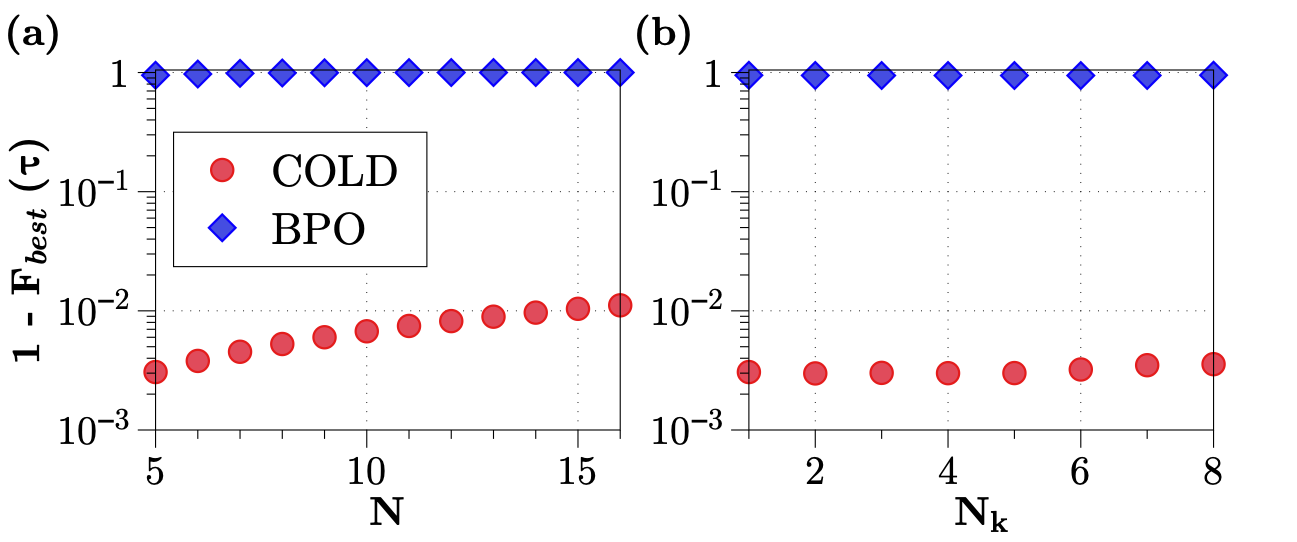
\includegraphics[width=0.8\linewidth]{images/ScalingN.png} \caption[Plots of how final state fidelities scale using COLD and BPO for different system sizes and optimisable parameters.]{Reproduced from \cite{cepaite_cold_2023}.}\label{fig:ising_maxamp}
\end{figure}

\begin{figure}[h]
    \centering
    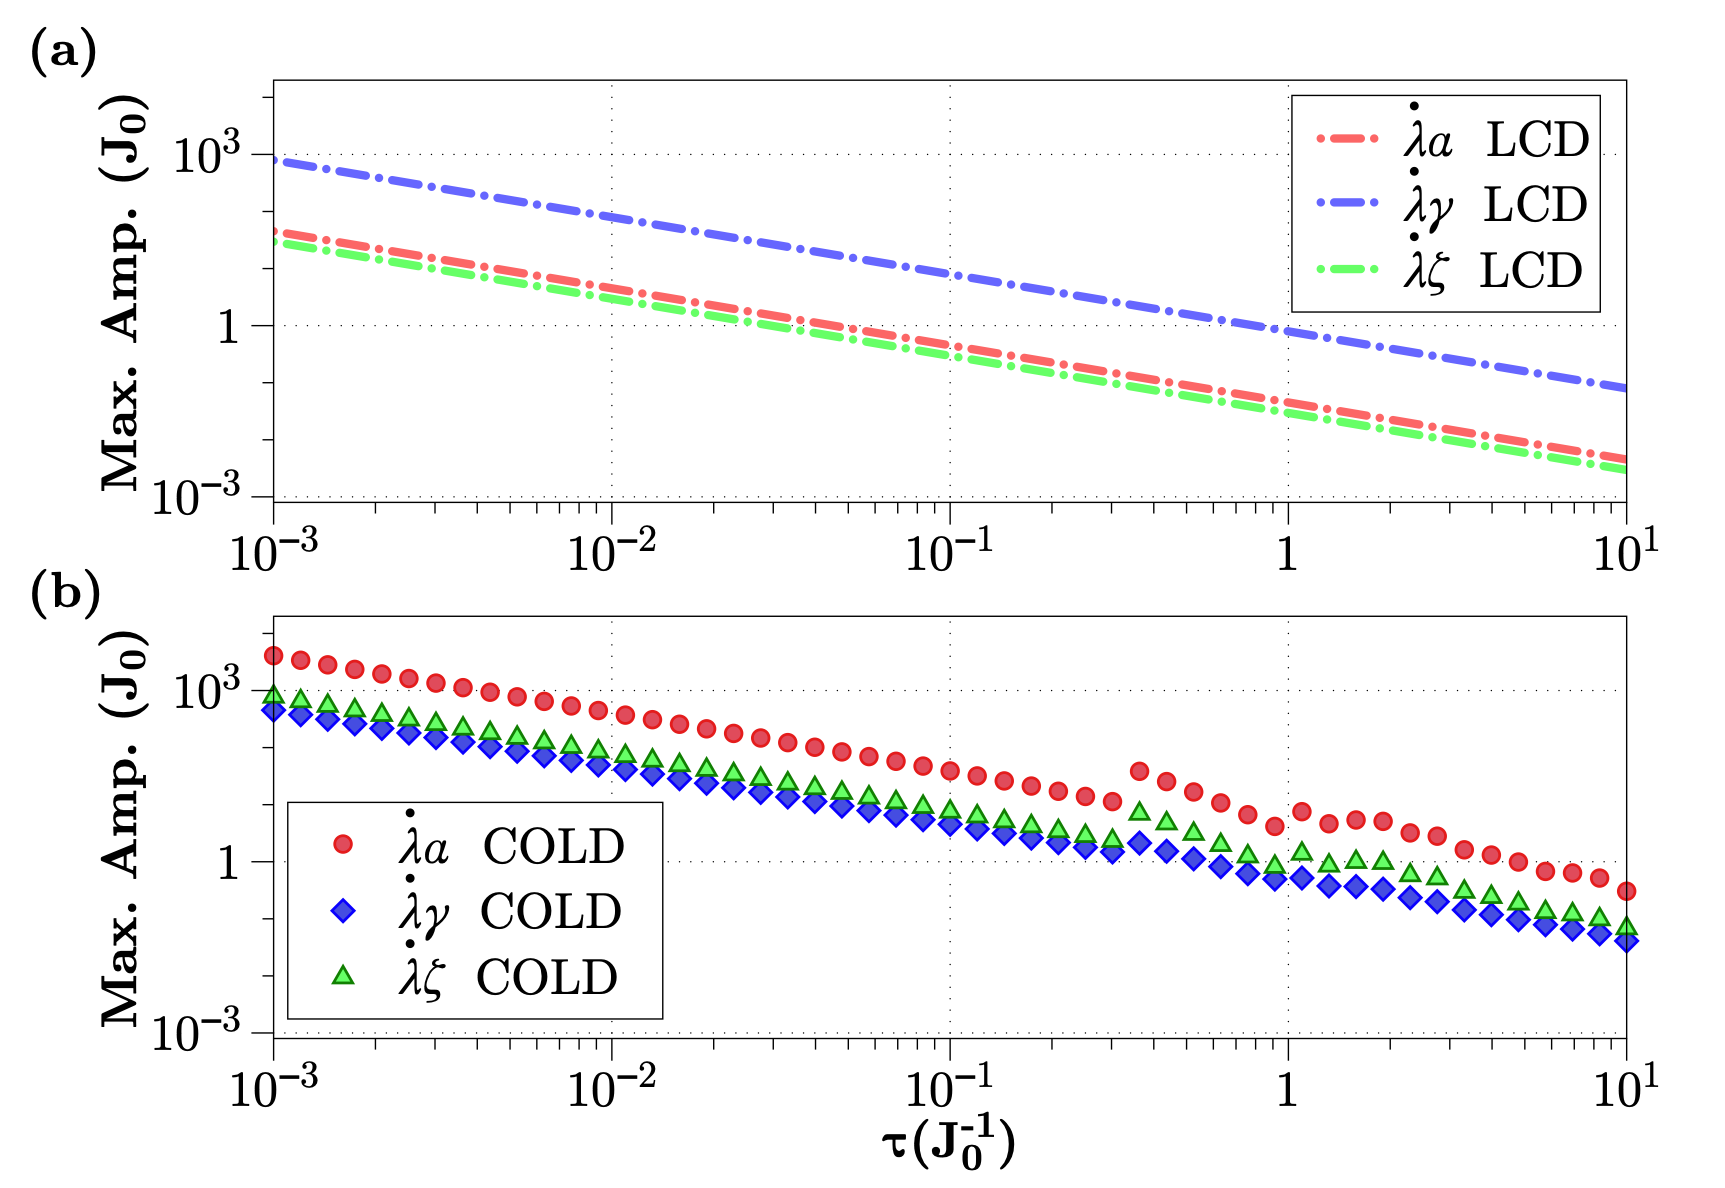
\includegraphics[width=0.8\linewidth]{images/MaxAmp.png} \caption[Plots of maximum amplitudes of LCD drives for the Ising spin chain.]{Reproduced from \cite{cepaite_cold_2023}.}\label{fig:ising_maxamp}
\end{figure}

\chapter{More details and plots for the higher order AGP chapter}\label{app:higher_order_AGP}

I have so much stuff to add here, might just leave some here for now. 


\begin{figure}[t]
\centering
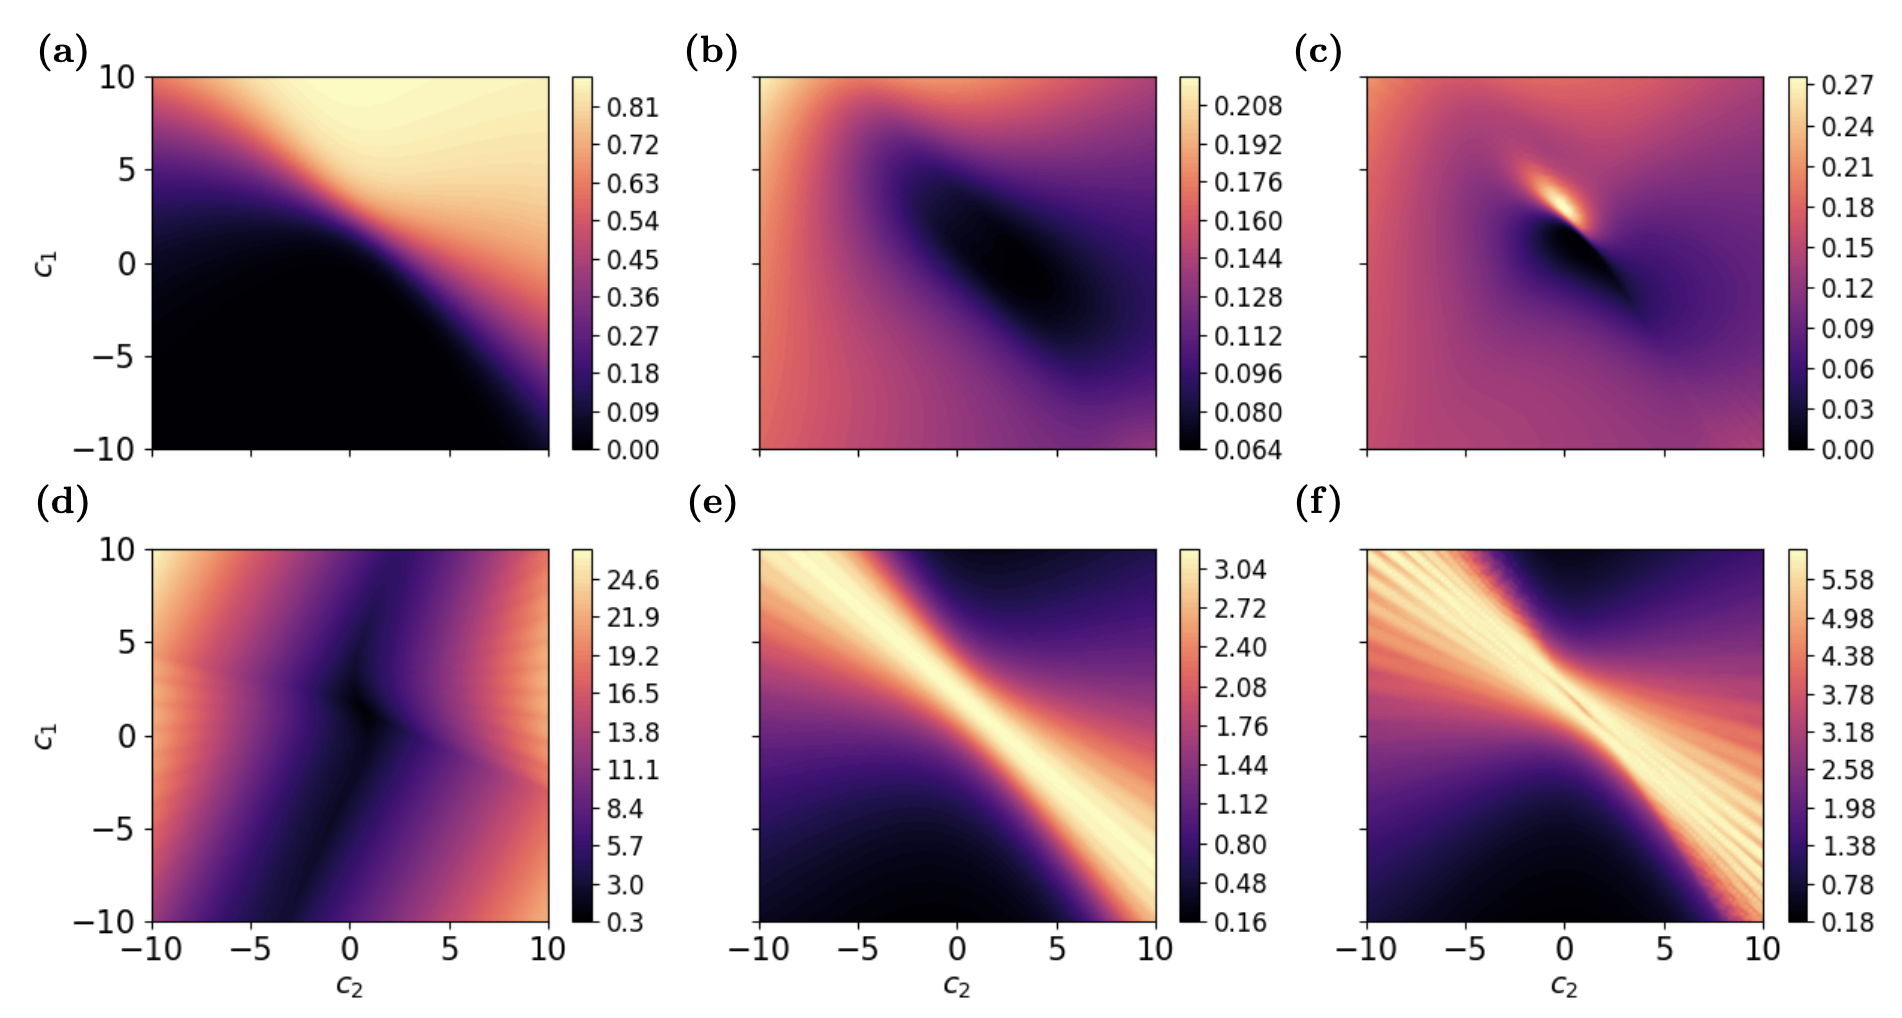
\includegraphics[width=\linewidth]{images/two_spin_contours_maxes.png} \caption{Placeholder: max amplitude scaled by Hamiltonian norm}\label{fig:}
\end{figure}


%%%%%%%%%%%%%%%%%%%%%%%%%%%%%%%%%%%%%%%%%%%%%%%%%%%%%%%%%%%%%%


%%%%%%%%%%%%%%%%%%%%%%%%%%%%%%%%%%%%%%%%%%%%%%%%%%%%%%%%%%%%%%
\addcontentsline{toc}{chapter}{Bibliography}
\bibliographystyle{util/ieeetran.bst}
\bibliography{references}

\end{document}